% !TEX root = ../Coherence.tex

\section{Categorical coherence} 
\label{s:catoperads}
 
\subsection{Basic definitions}

Throughout this section we consider structures without units.
Unless otherwise stated, the adjective "non-unital" will be implicitly assumed. 

\begin{definition} 
\label{def:catoperad}
A \emph{categorified non-symmetric operad} $\mathcal{P}$ is a collection $\left\{  \mathcal{P}(n)  \right\}_{n\in \mathbb{N}}$ of small categories equipped with bifunctors  
$$ \begin{array}{clll}
\circ_i&\colon& \mathcal{P}(n) \times
                    \mathcal{P}(k)
                    \longrightarrow \mathcal{P}(n+k-1) \ ,
                    & \text{for}\ 1 \leq i \leq n \ ,
\end{array}  $$
and for each $\kappa \in \mathcal{P}(m)$,  $\mu \in \mathcal{P}(n)$, $\nu \in \mathcal{P}(k)$, $1 \leq i \leq m$, $1 \leq j \leq n$ natural isomorphisms 
$$ \begin{array}{clll}
    \beta_{\kappa,\mu,\nu}&\colon& 
    (\kappa \circ_i \mu) \circ_{j+i-1} \nu  \overset{\cong}{\longrightarrow} \kappa \circ_i (\mu \circ_j \nu) \ , &  \\
    \theta_{\kappa,\nu,\mu}&\colon& 
    (\kappa \circ_i \nu) \circ_{j+k-1} \mu 
    \overset{\cong}{\longrightarrow} (\kappa \circ_j \mu) \circ_i \nu \ , & \text{when}\ i < j \ , 
\end{array}  $$
such that the following diagrams commute: the pentagonal \\
\resizebox{\linewidth}{!}{
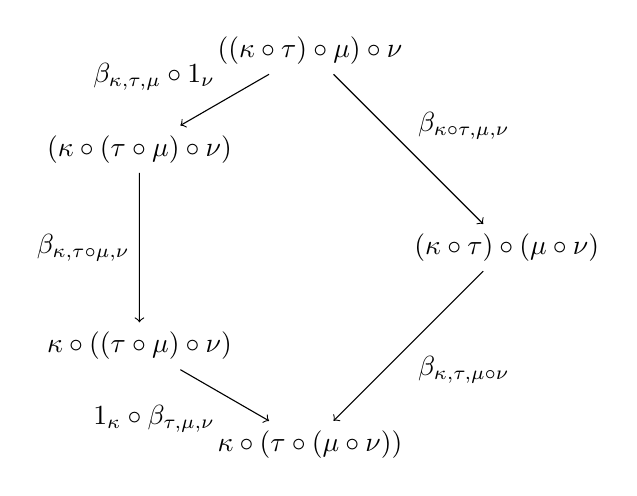
\begin{tikzpicture}[scale=2.5]
    \node (P1) at (0,1) {$((\kappa\circ\tau)\circ\mu)\circ\nu$};
    \node (P2) at (-0.866,0.5) {$(\kappa\circ(\tau\circ\mu)\circ\nu)$};
    \node (P3) at (-0.866,-0.5) {$\kappa\circ((\tau\circ\mu)\circ\nu)$};
    \node (P4) at (0,-1) {$\kappa\circ(\tau\circ(\mu\circ\nu))$};
    \node (P5) at (1,0) {$(\kappa\circ\tau)\circ(\mu\circ\nu)$} ;
    \draw[->] (P1)--(P2) node[midway,above left] {$\beta_{\kappa,\tau,\mu}\circ 1_\nu$};
    \draw[->] (P2)--(P3) node[midway,left] {$\beta_{\kappa,\tau\circ\mu,\nu}$};
    \draw[->] (P3)--(P4) node[midway,below left] {$1_\kappa \circ \beta_{\tau,\mu,\nu}$};
    \draw[->] (P1)--(P5) node[midway,above right] {$\beta_{\kappa\circ\tau,\mu,\nu}$};
    \draw[->] (P5)--(P4) node[midway,below right] {$\beta_{\kappa,\tau,\mu\circ\nu}$};
\end{tikzpicture} \quad 
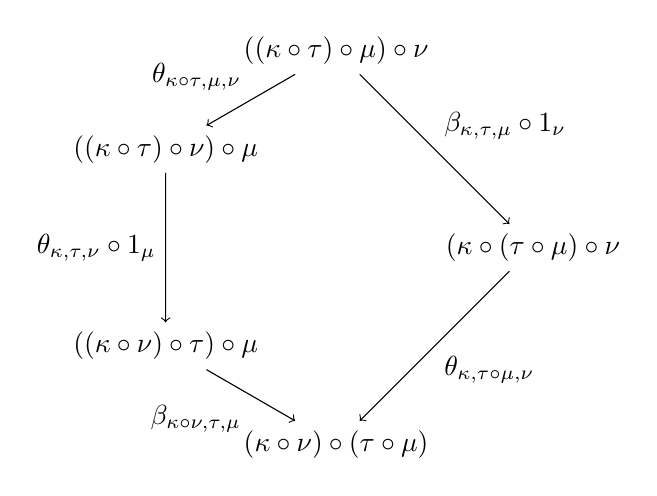
\begin{tikzpicture}[scale=2.5]
    \node (P1) at (0,1) {$((\kappa\circ\tau)\circ\mu)\circ\nu$};
    \node (P2) at (-0.866,0.5) {$((\kappa\circ\tau)\circ\nu)\circ\mu$};
    \node (P3) at (-0.866,-0.5) {$((\kappa\circ\nu)\circ\tau)\circ\mu$};
    \node (P4) at (0,-1) {$(\kappa\circ\nu)\circ(\tau\circ\mu)$};
    \node (P5) at (1,0) {$(\kappa\circ(\tau\circ\mu)\circ\nu$} ;
    \draw[->] (P1)--(P2) node[midway,above left] {$\theta_{\kappa\circ\tau,\mu,\nu}$};
    \draw[->] (P2)--(P3) node[midway,left] {$\theta_{\kappa,\tau,\nu}\circ 1_\mu$};
    \draw[->] (P3)--(P4) node[midway,below left] {$\beta_{\kappa\circ\nu,\tau,\mu}$};
    \draw[->] (P1)--(P5) node[midway,above right] {$\beta_{\kappa,\tau,\mu}\circ 1_\nu$};
    \draw[->] (P5)--(P4) node[midway,below right] {$\theta_{\kappa,\tau\circ\mu,\nu}$};
\end{tikzpicture} \quad 
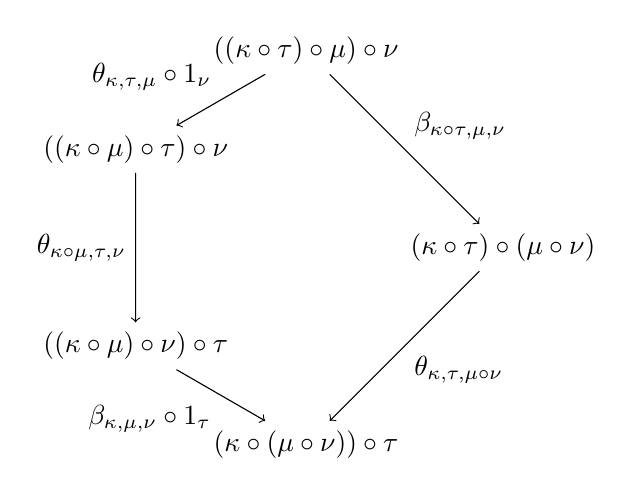
\begin{tikzpicture}[scale=2.5]
    \node (P1) at (0,1) {$((\kappa\circ\tau)\circ\mu)\circ\nu$};
    \node (P2) at (-0.866,0.5) {$((\kappa\circ\mu)\circ\tau)\circ\nu$};
    \node (P3) at (-0.866,-0.5) {$((\kappa\circ\mu)\circ\nu)\circ\tau$};
    \node (P4) at (0,-1) {$(\kappa\circ(\mu\circ\nu))\circ\tau$};
    \node (P5) at (1,0) {$(\kappa\circ\tau)\circ(\mu\circ\nu)$} ;
    \draw[->] (P1)--(P2) node[midway,above left] {$\theta_{\kappa,\tau,\mu}\circ 1_\nu$};
    \draw[->] (P2)--(P3) node[midway,left] {$\theta_{\kappa\circ\mu,\tau,\nu}$};
    \draw[->] (P3)--(P4) node[midway,below left] {$\beta_{\kappa,\mu,\nu}\circ 1_\tau$};
    \draw[->] (P1)--(P5) node[midway,above right] {$\beta_{\kappa\circ\tau,\mu,\nu}$};
    \draw[->] (P5)--(P4) node[midway,below right] {$\theta_{\kappa,\tau,\mu\circ\nu}$};
\end{tikzpicture} } \\
and hexagonal identities \\
\begin{center}
\resizebox{0.8\linewidth}{!}{
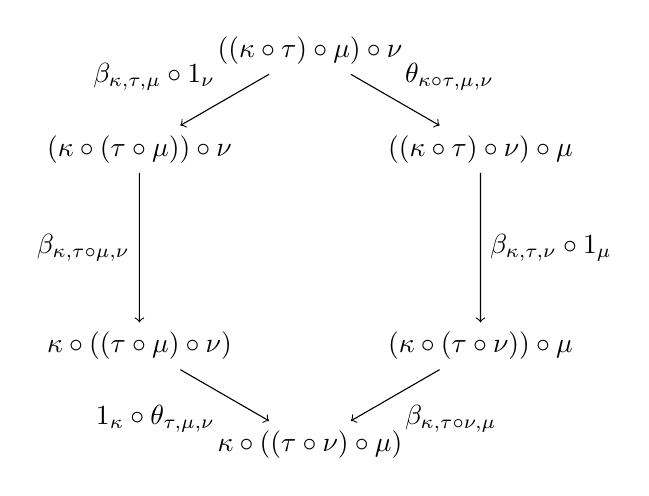
\begin{tikzpicture}[scale=2.5]
    \node (P1) at (0,1) {$((\kappa\circ\tau)\circ\mu)\circ\nu$};
    \node (P2) at (-0.866,0.5) {$(\kappa\circ(\tau\circ\mu))\circ\nu$};
    \node (P3) at (-0.866,-0.5) {$\kappa\circ((\tau\circ\mu)\circ\nu)$};
    \node (P4) at (0,-1) {$\kappa\circ((\tau\circ\nu)\circ\mu)$};
    \node (P5) at (0.866,0.5) {$((\kappa\circ\tau)\circ\nu)\circ\mu$} ;
    \node (P6) at (0.866,-0.5) {$(\kappa\circ(\tau\circ\nu))\circ\mu$};
    \draw[->] (P1)--(P2) node[midway,above left] {$\beta_{\kappa,\tau,\mu}\circ 1_\nu$};
    \draw[->] (P2)--(P3) node[midway,left] {$\beta_{\kappa,\tau\circ\mu,\nu}$};
    \draw[->] (P3)--(P4) node[midway,below left] {$1_\kappa \circ \theta_{\tau,\mu,\nu}$};
    \draw[->] (P1)--(P5) node[midway,above right] {$\theta_{\kappa\circ\tau,\mu,\nu}$};
    \draw[->] (P5)--(P6) node[midway,right] {$\beta_{\kappa,\tau,\nu}\circ 1_\mu$};
    \draw[->] (P6)--(P4) node[midway,below right] {$\beta_{\kappa,\tau\circ\nu,\mu}$};
\end{tikzpicture} \quad \quad
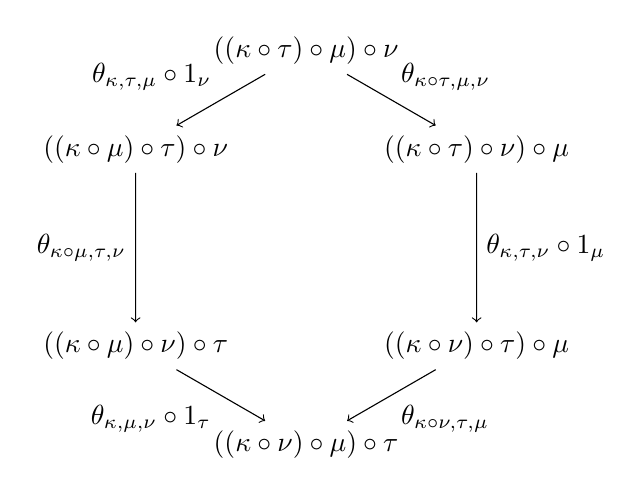
\begin{tikzpicture}[scale=2.5]
    \node (P1) at (0,1) {$((\kappa\circ\tau)\circ\mu)\circ\nu$};
    \node (P2) at (-0.866,0.5) {$((\kappa\circ\mu)\circ\tau)\circ\nu$};
    \node (P3) at (-0.866,-0.5) {$((\kappa\circ\mu)\circ\nu)\circ\tau$};
    \node (P4) at (0,-1) {$((\kappa\circ\nu)\circ\mu)\circ\tau$};
    \node (P5) at (0.866,0.5) {$((\kappa\circ\tau)\circ\nu)\circ\mu$} ;
    \node (P6) at (0.866,-0.5) {$((\kappa\circ\nu)\circ\tau)\circ\mu$};
    \draw[->] (P1)--(P2) node[midway,above left] {$\theta_{\kappa,\tau,\mu}\circ 1_\nu$};
    \draw[->] (P2)--(P3) node[midway,left] {$\theta_{\kappa\circ\mu,\tau,\nu}$};
    \draw[->] (P3)--(P4) node[midway,below left] {$\theta_{\kappa,\mu,\nu}\circ 1_\tau$};
    \draw[->] (P1)--(P5) node[midway,above right] {$\theta_{\kappa\circ\tau,\mu,\nu}$};
    \draw[->] (P5)--(P6) node[midway,right] {$\theta_{\kappa,\tau,\nu}\circ 1_\mu$};
    \draw[->] (P6)--(P4) node[midway,below right] {$\theta_{\kappa\circ\nu,\tau,\mu}$};
\end{tikzpicture}  } \quad \ .
\end{center}
\end{definition}
The diagrams above hold for all instances of composable $\beta$ and $\theta$; these depend on the indices $i,j,k$, which are omitted for the sake of readability. 
Observe that a categorified non-symmetric operad concentrated in arity $1$ is a non-symmetric monoidal category.

\begin{rem}
\label{rem:DPLA}
K. Do{\v s}en and Z. Petri{\'c} introduce in \cite[Section 12]{DP15} the notion of weak Cat-operad.
Despite looking different at first sight, the two notions are in fact equivalent.
The crucial observation is the following: the $\theta$-isomorphisms of Do{\v s}en--Petri{\'c} comprise both the isomorphisms~$\theta$ in \cref{def:catoperad} and their inverses $\theta^{-1}$.
Therefore, there are only two pentagonal coherence diagrams in the definition of a weak Cat-operad, the equations ($\beta$ $pent_e$) and ($\beta\theta 2_e$) of \cite[Section 9]{DP15}.
The set of diagrams of the form ($\beta$ $pent_e$) is the same as the set of diagrams which arises from the first pentagon in \cref{def:catoperad}, while the set of diagrams of the form ($\beta\theta 2_e$) is partitioned into the sets of diagrams which arise from the second and third pentagons in \cref{def:catoperad}.
\end{rem}

\begin{definition}
    A \emph{strong morphism of categorified non-symmetric operads} $F: \mathcal{P} \to \mathcal{Q}$ is a collection of functors $F_n : \mathcal{P}(n) \to \mathcal{Q}(n)$ together with natural isomorphisms $\gamma_{\kappa,\mu}: F_{m-1+n}(\kappa \circ_i \mu) \overset{\cong}{\longrightarrow} F_m(\kappa) \circ_i F_n(\mu)$ such that the following diagrams commute:
    \begin{center}
    \resizebox{0.8\linewidth}{!}{
    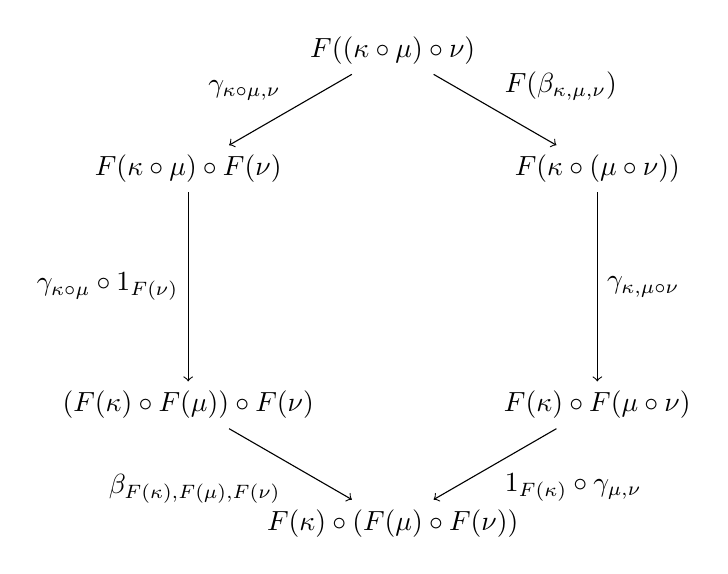
\begin{tikzpicture}[scale=3]
        \node (P1) at (0,1) {$F((\kappa\circ\mu)\circ\nu)$};
        \node (P2) at (-0.866,0.5) {$F(\kappa\circ\mu)\circ F(\nu)$};
        \node (P3) at (-0.866,-0.5) {$(F(\kappa)\circ F(\mu))\circ F(\nu)$};
        \node (P4) at (0,-1) {$F(\kappa)\circ(F(\mu)\circ F(\nu))$};
        \node (P5) at (0.866,0.5) {$F(\kappa\circ(\mu\circ\nu))$} ;
        \node (P6) at (0.866,-0.5) {$F(\kappa)\circ F(\mu\circ\nu)$};
        \draw[->] (P1)--(P2) node[midway,above left] {$\gamma_{\kappa\circ\mu,\nu}$};
        \draw[->] (P2)--(P3) node[midway,left] {$\gamma_{\kappa\circ\mu}\circ 1_{F(\nu)}$};
        \draw[->] (P3)--(P4) node[midway,below left] {$\beta_{F(\kappa),F(\mu),F(\nu)}$};
        \draw[->] (P1)--(P5) node[midway,above right] {$F(\beta_{\kappa,\mu,\nu})$};
        \draw[->] (P5)--(P6) node[midway,right] {$\gamma_{\kappa,\mu\circ\nu}$};
        \draw[->] (P6)--(P4) node[midway,below right] {$1_{F(\kappa)}\circ\gamma_{\mu,\nu}$};
    \end{tikzpicture}  \quad \quad
    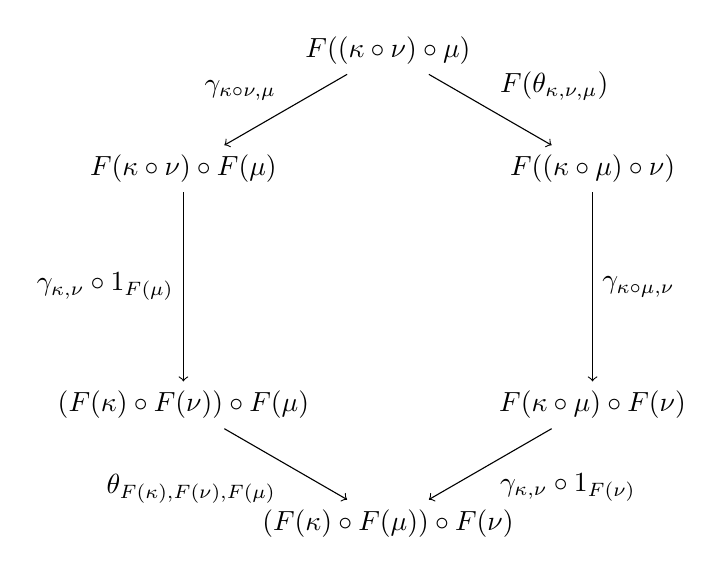
\begin{tikzpicture}[scale=3]
        \node (P1) at (0,1) {$F((\kappa\circ\nu)\circ\mu)$};
        \node (P2) at (-0.866,0.5) {$F(\kappa\circ\nu)\circ F(\mu)$};
        \node (P3) at (-0.866,-0.5) {$(F(\kappa)\circ F(\nu))\circ F(\mu)$};
        \node (P4) at (0,-1) {$(F(\kappa)\circ F(\mu))\circ F(\nu)$};
        \node (P5) at (0.866,0.5) {$F((\kappa\circ\mu)\circ\nu)$} ;
        \node (P6) at (0.866,-0.5) {$F(\kappa\circ\mu)\circ F(\nu)$};
        \draw[->] (P1)--(P2) node[midway,above left] {$\gamma_{\kappa\circ\nu,\mu}$};
        \draw[->] (P2)--(P3) node[midway,left] {$\gamma_{\kappa,\nu}\circ 1_{F(\mu)}$};
        \draw[->] (P3)--(P4) node[midway,below left] {$\theta_{F(\kappa),F(\nu),F(\mu)}$};
        \draw[->] (P1)--(P5) node[midway,above right] {$F(\theta_{\kappa,\nu,\mu})$};
        \draw[->] (P5)--(P6) node[midway,right] {$\gamma_{\kappa\circ\mu,\nu}$};
        \draw[->] (P6)--(P4) node[midway,below right] {$\gamma_{\kappa,\nu}\circ 1_{F(\nu)}$};
    \end{tikzpicture}  } \quad \ .
\end{center}
    It is said to be \emph{strict} if the natural isomorphisms are identities. 
\end{definition}

Once again, the diagrams above hold for all instances of $\beta$ and $\theta$ arrows, and we have omitted the $(i,j,k)$-indices for readability. 
Observe that a strong (resp. strict) morphism between categorified non-symmetric operads concentrated in arity $1$ is a strong (resp. strict) monoidal functor between non-symmetric monoidal categories. 

\subsection{Coherence theorem}

We now aim at the coherence theorem for categorified non-symmetric operads.
In order to state the theorem, we construct the free non-symmetric categorified operad on a family of sets $S=\{S_n\}_{n \geq 1}$.
We define a family of groupoids $\mathcal{S}=\{\mathcal{S}_n\}_{n \geq 1}$ whose objects are given by the following rules:
\begin{enumerate}
    \item if $\mu \in S_n$, then $\mu$ is an object of $\mathcal{S}_n$;
    \item if $\mu \in \mathcal{S}_m$ and $\nu \in \mathcal{S}_n$, then $\mu \circ_i \nu$ is an object of $\mathcal{S}_{m-1+n}$, for any $1 \leq i \leq m$.
\end{enumerate}
Now we define a set $M$ of basic morphisms $\id_\mu : \mu \to \mu$ for all objects $\mu\in \mathcal{S}$, $\beta: (\kappa \circ_i \mu) \circ_{j+i-1} \nu \leftrightarrow \kappa \circ_i (\mu \circ_j \nu) : \beta^{-1}$ for every $\kappa \in \mathcal{S}_m, \mu \in \mathcal{S}_n, \nu \in \mathcal{S}_k$, $1 \leq i \leq m$ and $1 \leq j \leq n$, and $\theta: (\kappa \circ_i \nu) \circ_{j-1+k} \mu \leftrightarrow (\kappa \circ_j \mu) \circ_i \nu : \theta^{-1}$ whenever $i<j$.
We then define the morphisms of the family $\mathcal{S}$ by the following rules:
\begin{enumerate}
    \item if $\phi \in M$, then $\phi$ is a morphism of $\mathcal{S}$; 
    \item if $\phi_1: t_1 \to t_2$ and $\phi_2: t_2 \to t_3$ are morphisms of $\mathcal{S}$, then so is $\phi_2 \phi_1 : t_1 \to t_3$;
    \item if $\phi : t_1 \to t_2$ is a morphism in $\mathcal{S}_m$, and $t_3 \in \mathcal{S}_n$, then $\phi \circ_i \id : t_1 \circ_i t_3 \to t_2 \circ_i t_3$ is a morphism for any $1 \leq i \leq m$, and $\id \circ_j \phi : t_3 \circ_j t_1 \to t_3 \circ_j t_2$ is a morphism for any $1 \leq j \leq n$. 
\end{enumerate}
This finishes the construction of our family of groupoids $\mathcal{S}$.

One can think about the objects of $\mathcal{S}$ as the set of fully nested planar trees \cite[Definition 2.2]{laplante-anfossiDiagonalOperahedra2022a} whose vertices are decorated by objects of $S$, subject to the requirement that if a vertex has $n$ incoming edges, it must be decorated by an element of $S_n$. 
The nestings in the tree represent the order in which the objects decorating the vertices should be formally composed, as represented in \cref{fig:treeandnesting}.
Morphisms in $\mathcal{S}$ are sequences of applications of the associativity rules $\beta$ and $\theta$, moving one nest at a time to a neighbouring pair of vertices. 

\begin{figure}[h!]
\centering
\resizebox{0.4\linewidth}{!}{
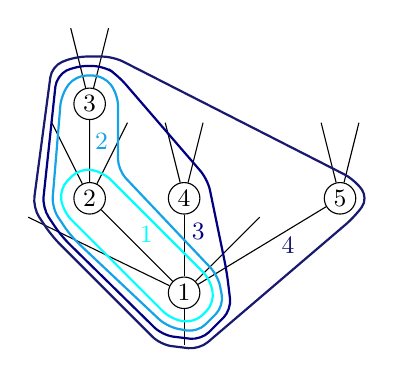
\begin{tikzpicture}[scale=1.2]
        \node (E)[circle,draw=black,minimum size=4mm,inner sep=0.1mm] at (-0,0) {\small $1$};
        \node (F) [circle,draw=black,minimum size=4mm,inner sep=0.1mm] at (-1,1) {\small $2$};
        \node (A) [circle,draw=black,minimum size=4mm,inner sep=0.1mm] at (-1,2) {\small $3$};
        \node (q) [circle,draw=black,minimum size=4mm,inner sep=0.1mm] at (0,1) {\small $4$};
        \node (r) [circle,draw=black,minimum size=4mm,inner sep=0.1mm] at (1.65,1) {\small $5$};
        \node (x) [circle,draw=none,minimum size=4mm,inner sep=0.1mm] at (-0.4,0.62) {\color{Cyan} \small $1$};
        \node (y) [circle,draw=none,minimum size=4mm,inner sep=0.1mm] at (-0.875,1.6) {\color{Cerulean} \small $2$};
        \node (u) [circle,draw=none,minimum size=4mm,inner sep=0.1mm] at (0.15,0.65) {\color{NavyBlue} \small $3$};
        \node (v) [circle,draw=none,minimum size=4mm,inner sep=0.1mm] at (1.1,0.5) {\color{MidnightBlue} \small $4$};
        \draw[-] (0.8,0.8) -- (E)--(-1.65,0.8); 
        \draw[-] (-1.2,2.8) -- (A)--(-0.8,2.8); 
        \draw[-] (-0.2,1.8) -- (q)--(0.2,1.8);   
        \draw[-] (1.85,1.8) -- (r)--(1.45,1.8); 
        \draw[-] (E)--(0,-0.55); 
        \draw[-] (-1.4,1.8) -- (F)--(-0.6,1.8);   
        \draw[-] (E)--(F) node {};
        \draw[-] (E)--(q) node  {};
        \draw[-] (E)--(r) node {};
        \draw[-] (F)--(A) node {};
        \draw [Cyan,rounded corners,thick] (0.11,-0.32) -- (-0.14,-0.28) -- (-1.28,0.86) -- (-1.32,1.1) --  (-1.1,1.32) -- (-0.86,1.28) -- (0.28,0.14) -- (0.32,-0.11) -- cycle;
        \draw [Cerulean,rounded corners,thick] (0.14,-0.42) -- (-0.18,-0.36) -- (-1.2,0.6) -- (-1.4,0.9) -- (-1.3,2.1) -- (-1.15,2.3) -- (-0.85,2.3) -- (-0.7,2.1) --  (-0.7,1.3) -- (0.36,0.18) -- (0.42,-0.14) -- cycle;
        \draw [NavyBlue,rounded corners,thick] (0.18,-0.5) -- (-0.23,-0.45) -- (-1.3,0.6) -- (-1.5,0.9) --  (-1.35,2.3) --  (-1.15,2.4) --  (-0.85,2.4) --  (-0.7,2.3) --  (.25,1.2) -- (0.45,0.23) -- (0.5,-0.18) -- cycle;
        \draw [MidnightBlue,rounded corners,thick] (0.16,-0.6) -- (-0.25,-0.55) -- (-1.4,0.6) -- (-1.6,0.9) --  (-1.4,2.4) --  (-1.15,2.5) --  (-0.75,2.5) --  (1.8,1.2) --  (1.95,1) --  (1.8,0.8) -- cycle;
\end{tikzpicture} }
\caption{A fully nested planar tree.}
\label{fig:treeandnesting}
\end{figure} 

\begin{definition}
    We denote by $\mathcal{F}(S)$ the quotient of the family of groupoids $\mathcal{S}$ by the axioms of bifunctors, and the coherence diagrams defining a categorified non-symmetric operad. 
\end{definition}

\begin{rem}
    In the tree representation for $\mathcal{S}$, there is a coherence diagram for every decorated planar tree with 4 vertices \cite[p.258]{curienSyntacticAspectsHypergraph2019a}.
    In the rewriting system formed by the fully nested planar trees and the $\beta$ and $\theta$ arrows, these correspond precisely to the critical pairs \cite[Section 6.2]{baaderTermRewritingAll1998}.
\end{rem}

We obtain that $\mathcal{F}(S)$ is the free categorified non-symmetric operad on $S$. 
That is, for any categorified non-symmetric operad $\mathcal{P}$, and for family of functions $\rho_n : S_n \to \obj(\mathcal{P}(n))$, there is a unique strict morphism of non-symmetric categorified operads $[-]:\mathcal{F}(S) \to \mathcal{P}$ that extends $\rho=\{\rho_n\}_{n\geq 1}$. 

\begin{thm}[Coherence theorem]
\label{thm:coherence-operahedra}
    For any categorified non-symmetric operad $\mathcal{P}$, for any family of functions $\rho : S \to \obj(P)$, and for any two parallel morphisms $\phi_1,\phi_2: t_1 \to t_2$ in $\mathcal{F}(S)$, we have $[\phi_1]=[\phi_2]$.
\end{thm}

\begin{proof}
The morphisms of $\mathcal{S}$ are in bijection with combinatorial paths on a family of polytopes called operahedra \cite[Section 2.1]{laplante-anfossiDiagonalOperahedra2022a}, see also \cite[Section 13]{DP15} and \cite{curienSyntacticAspectsHypergraph2019a}, whose faces are in bijection with the set of all nestings on a planar tree. 
There is one operahedron for each planar tree $t$, and its vertices are in bijection with the maximal nestings of~$t$. 
Two parallel morphisms in $\mathcal{S}$ thus define two parallel combinatorial parths on some operahedron. 
Since an operahedron is simply connected, \cref{thm:top-coherence} implies that these two combinatorial paths are combinatorially homotopic. 
The result then follows from the fact that a $2$-face of an operahedron is exactly either a square (witnessing naturality), a pentagon or an hexagon (witnessing a coherence condition) as in \cref{def:catoperad} above.
\end{proof}

\begin{proof}[Second proof]
    Alternatively, since the operahedra are polytopes, one can use \cref{p:second-proof}. 
    Choosing a generic vector $\vec v$ which has strictly decreasing coordinates for the Loday realizations \cite[Section 2.2]{laplante-anfossiDiagonalOperahedra2022a} gives the orientations of the diagrams given in \cref{def:catoperad} on every $2$-face \cite[Proposition 3.11]{laplante-anfossiDiagonalOperahedra2022a}.
    The posets/rewriting system obtained generalize the Tamari lattice on fully nested linear trees \cite[Definition 2.8]{laplante-anfossiDiagonalOperahedra2022a}.
    One then obtains a topological proof of coherence which is almost word for word the original proof of MacLane \cite[Theorem 3.1]{MacLane63}, suitably generalized to categorified operads. 
\end{proof}
   
Following \cref{rem:DPLA}, we have that \cref{thm:coherence-operahedra} gives an alternative, more economical proof of coherence for weak Cat-operads \cite[Proposition 14.2]{DP15}.
Incidentally, it gives an alternative input to the proof of coherence for cyclic symmetric categorified operads \cite{curienCategorifiedCyclicOperads2020}.

Restricting the theorem above to non-symmetric operads concentrated in arity $1$, the category $\mathcal{F}(S)$ becomes the free non-symmetric monoidal category on $S$, and we get the following corollary. 

\begin{corollary}[MacLane's coherence theorem for non-symmetric monoidal categories]
\label{cor:MacLane}
    For any non-symmetric monoidal category $\mathcal{C}$, for any function $\rho : S \to \obj(\mathcal{C})$, and for any two parallel morphisms $\phi_1,\phi_2: t_1 \to t_2$ in $\mathcal{F}(S)$, we have $[\phi_1]=[\phi_2]$.
\end{corollary}

\subsection{Symmetric monoidal categories} 
One can use the same ideas to prove MacLane's coherence theorem for \emph{symmetric} monoidal categories, using the family of permutoassociahedra \cite{kapranov1993,reinerCoxeterassociahedra1994}. 
Here we simply formulate the theorem, the proof is really the same as the one of \cref{thm:coherence-operahedra}.

Let $W_n$ denote the set of non-commutative, fully parenthesized words on $n$ distinct letters. 
Let $(\mathcal{C}, \otimes)$ be a symmetric monoidal category.
Each $w \in W_n$ defines in an obvious way a functor $[w] : \mathcal{C}^{\times n} \to \mathcal{C}$.
For instance, if $w=((ab)c)(ed)$, then the associated functor is defined on objects and morphisms by the formula
\begin{eqnarray*}
    [w] \quad : \quad \mathcal{C}^{\times n} & \to & \mathcal{C} \\
    (a,b,c,d,e) & \mapsto & ((a \otimes b) \otimes c)\otimes (e \otimes d) \ .
\end{eqnarray*}
We consider the groupoid $\mathcal{W}_n$ which has objects the elements of $W_n$, and morphisms generated by the ones of the form $\phi : w_1 \to w_2$, where the word $w_2$ is obtained from $w_1$ by applying either $\alpha : ((ww')w'') \to (w(w'w''))$ or $\tau : ab \to ba$ to a subword of $w_1$.
To any such $\phi$ one can associate a natural transformation $[\phi] : [w_1] \to [w_2]$ in the obvious way. 

\begin{thm}[MacLane's coherence theorem]
    \label{thm:MacLane}
    For any symmetric monoidal category $\mathcal{C}$, and for any pair of parallel morphisms $\phi_1,\phi_2: w_1 \to w_2$ in $\mathcal{W}=\{\mathcal{W}_n\}_{n\geq 1}$, we have $[\phi_1]=[\phi_2]$.
\end{thm}

\subsection{Further applications} 
\label{sec:further}
One can also use the same strategy to prove coherence theorem \emph{unital} non-symmetric monoidal categories, using the unital associahedra of F. Muro and A. Tonks \cite{muroUnitalAssociahedra2014}.

It is natural to ask if the construction of unital associahedra could be extended to the permutoassociahedra, in such a way as to provide a topological proof of coherence for unital symmetric monoidal categories. 
The question of the existence of these constructions at the operadic level (i.e. does there exist unital operahedra, symmetric operahedra, and unital symmetric operahedra?) is, to our knowledge, still open as well. 

Another immediate application of \cref{thm:top-coherence} is the coherence of strong non-symmetric monoidal functors between non-symmetric monoidal categories \cite{epsteinFunctorsTensoredCategories1966}. 
The corresponding topological objects are in this case the family of multiplihedra \cite{Stasheff70,Forcey08}.
The generalization to strong morphisms between non-symmetric categorified operads also goes through, involving this time the family of multiploperahedra described at the end of the introduction in \cite{MazuirLA22}.

In the same spirit as in \cref{thm:coherence-operahedra}, one could obtain coherence results for categorifications of many operad-like structures, for instance the ones described in \cite{BMO20}: categorified modular operads, wheeled properads, and permutads (shuffle algebras), among others.
In order to treat cyclic and symmetric structures, one could take inspiration from the reduction process followed in \cite{curienCategorifiedCyclicOperads2020} for the case of cyclic symmetric categorified operads.

